\chapter{Introduction}
\label{ch:introduction}

E-commerce has been around for a number of decades by now. Since the release of the Netscape browser in 1994 companies have been selling their products online. From 1995 to 2000 the number of companies who were selling their products online increased significantly. Venture capitalists invested huge amounts of money in these new internet companies. Sadly, the excitement wasn’t well founded. The world wasn’t ready for a shift from traditional retailing to e-commerce. People were wary about ordering products online, online payment methods weren’t very widely accepted and parcel services weren’t optimized for delivering the products to the people.

The excitement about internet companies led to the dotcom bubble bursting in 2000. A lot of new internet companies went bankrupt, others had to downsize significantly. A lot of survivors of the dotcom bubble are still around today. They have now become huge internet companies, some examples are: amazon.com, ebay.com and dell.com.

In the last 15 years online retailing has been steadily increasing. People were getting more comfortable buying their products online, online payment methods improved significantly and parcel services optimized their distribution network. These improvements gave small companies the opportunity to start selling their products online.
The speed at which ecommerce is cutting into traditional retail’s market share is incredible. Q1 2010 saw just 4.2\% of US retail sales happening online. In Q1 2019 that was 10.5\%. The pandemic and subsequent lock-downs took that to 16.1\% in Q2 2020.

It’s worth noting that the pandemic has accelerated consumer adoption of e-commerce, and this growth looks to be exponential. It’s expected that 95\% of the global retail market will be happening online by 2040. \cite{RetailVsEcom2022}

\section{Course content}
In this course you will learn to create and manage a web store. There are a lot of platforms which allow you to create a web store. In this course we chose to use Drupal. Drupal is a content management system (CMS) written in PHP. It has many features that will make it easy to create a web store.

First we’ll learn how to create, manage and edit a basic Drupal site. Afterwards we’ll add the web store functionality through the use of modules. During the course you’ll also learn how to write PHP code, manage your site through git, collaborate on your site and deploy it to a server.

\section{What is a CMS?}
Drupal is a content management system or CMS. The name is a good description of what it actually does. It’s an application which makes it easy to manage content. The content can be of different types. For example, a blog can use a CMS. The type of content on the blog will be articles. The CMS makes it easy to create, edit, remove and manage articles. Another example where a CMS can be useful is when you create a web store. The type of content we use here are products. The CMS makes it easy to manage the products, for example: add a product, change the price or add a shipping method.
A lot of big websites use a CMS as their background application. Examples include: www.engadget.com, www.puma.com, www.societegenerale.com. Figure \ref{fig:cms_systems} shows different CMS systems.

\begin{figure}[h]
    \centering
    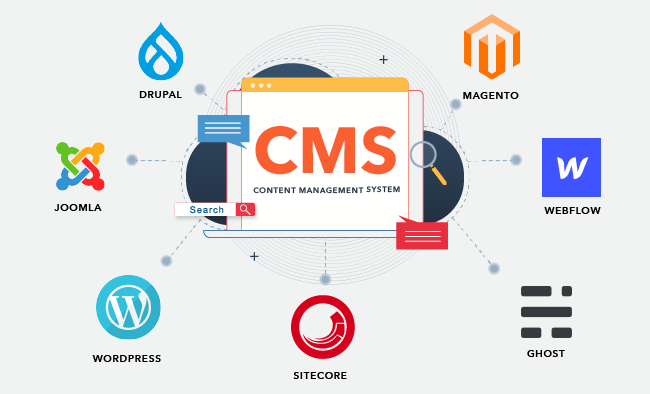
\includegraphics[width=1\linewidth]{img/ch1/cms_systems}
    \caption{A lot of different CMS systems are available on the market, Drupal being one of them \cite{HubSpot2022}}
    \label{fig:cms_systems}
\end{figure}



\section{What is Drupal?}
As mentioned before, Drupal (logo figure 1.2) is an open source CMS written in PHP. Drupal is web based so it uses HTML, CSS and JavaScript as application front end. A Drupal application is completely customizable. We can change the look of our site by changing the HTML and CSS (Drupal calls this theming).
The application back end can be extended by adding our own code or code other people made available online (Drupal does this through its module system).
Drupal was created in 2001 by Dries Buytaert. He got his degree in computer science at the university of Antwerp and his PhD at Ghent university. In 2007 he started the company Acquia which provides services to organizations using Drupal as their CMS. In 2009 Acquia helped with the relaunch of Whitehouse.gov. Next to whitehouse.gov a lot of other sites use Drupal. At https://www.drupal.com/showcases you can find a list of different sites build with Drupal.

\subsection{Drupal 9}
Drupal 9 is released on June 3, 2020, which builds on the same base as Drupal 8. Drupal 9 is a cleaned-up version of Drupal 8. It is the same as the last Drupal 8 minor version with our own deprecated code removed and third-party dependencies updated. Most extensions will only need a few changes.

\section{Review Exercise}
\begin{enumerate}
    \item Look up the definition of a CMS on Wikipedia.
    \item Think of five content types that could be managed by a CMS.
    \item Find five sites which use Drupal as CMS.
    \item Name three other content management systems.
\end{enumerate}
